\documentclass{standalone}

\usepackage{tikz}
    \usetikzlibrary{arrows, arrows.meta}
    \usetikzlibrary{calc}
    \usetikzlibrary {decorations.pathmorphing}
    
\tikzset{
    bluearrow/.style={
        blue!25,
        -{Kite[length=2.5mm]}, 
        line width=0.5mm,},
    greensq/.style={
        green,
        fill=green!20, 
        line width=0.4mm,},
    redsq/.style={
        red,
        fill=red!20, 
        line width=0.4mm,},
    }

\begin{document}
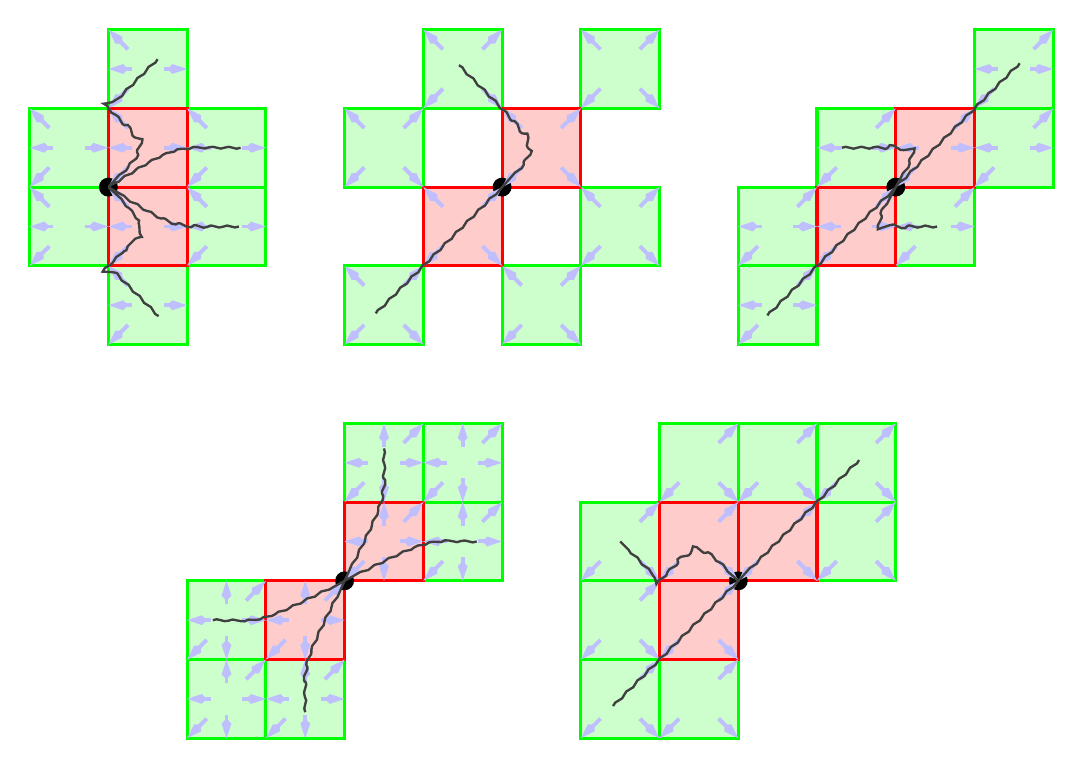
\begin{tikzpicture}
    % \draw[help lines] (0,-5) grid (13,4);
    \foreach \x in % green
        {(0,1), (0,2), (1,0), (2,1), (2,2), (1,3), % case (A)
         (4,0), (6,0), (7,1), (4,2), (5,3), (7,3), % case (B)
         (9,0), (9,1), (11,1), (10,2), (12,2), (12,3), % case (C)
         (3,-5), (2,-4), (5,-3), (4,-2), (5,-2), (2,-5), % case (D6)
         (7,-5), (8,-5), (7,-4), (7,-3), (10,-3), (8,-2), (9,-2), (10,-2) % case (D3)
        } 
        {\draw[greensq] \x rectangle+(1,1);} 
    \foreach \x in % red
        {(1,1), (1,2), % case (A)
         (5,1), (6,2), % case (B)
         (10,1), (11,2), % case (C)
         (3,-4), (4,-3), % case (D6)
         (8,-4), (8,-3), (9,-3) % case (D3)
        } 
        {\draw[redsq] \x rectangle+(1,1);} 
    \fill[black] 
        (1,2) circle (1.2mm)
        (6,2) circle (1.2mm)
        (11,2) circle (1.2mm)
        (4,-3) circle (1.2mm)
        (9,-3) circle (1.2mm);
    % case (A) bound
    \foreach \x in
        {(0,1), (0,2), (1,0), (2,1), (2,2), (1,3), (1,1), (1,2)} 
        {\draw[bluearrow] \x++(0.25,0.75) -- ++(-.25,0.25);
         \draw[bluearrow] \x++(0.25,0.25) -- ++(-0.25,-0.25);
         \draw[bluearrow] \x++(0.3,0.5) -- ++(-0.3,0);
         \draw[bluearrow] \x++(0.7,0.5) -- ++(0.3,0);}
    % case (B) bound
    \foreach \x in
        {(4,0), (6,0), (7,1), (4,2), (5,3), (7,3), (5,1), (6,2)} 
        {\draw[bluearrow] \x++(0.25,0.75) -- ++(-.25,0.25);
         \draw[bluearrow] \x++(0.25,0.25) -- ++(-0.25,-0.25);
         \draw[bluearrow] \x++(0.75,0.75) -- ++(.25,0.25);
         \draw[bluearrow] \x++(0.75,0.25) -- ++(0.25,-0.25);}
    % case (C) bound
    \foreach \x in
        {(9,0), (9,1), (11,1), (10,2), (12,2), (12,3),(10,1), (11,2)} 
        {\draw[bluearrow] \x++(0.25,0.25) -- ++(-0.25,-0.25);
         \draw[bluearrow] \x++(0.75,0.75) -- ++(.25,0.25);
         \draw[bluearrow] \x++(0.3,0.5) -- ++(-0.3,0);
         \draw[bluearrow] \x++(0.7,0.5) -- ++(0.3,0);}
    % case (D6) bound
    \foreach \x in
        { (3,-5), (2,-4), (5,-3), (4,-2), (4,-3), (3,-4), (5,-2), (2,-5)} 
        {\draw[bluearrow] \x++(0.25,0.25) -- ++(-0.25,-0.25);
         \draw[bluearrow] \x++(0.75,0.75) -- ++(.25,0.25);
         \draw[bluearrow] \x++(0.3,0.5) -- ++(-0.3,0);
         \draw[bluearrow] \x++(0.7,0.5) -- ++(0.3,0);
         \draw[bluearrow] \x++(0.5,0.3) -- ++(0,-0.3);
         \draw[bluearrow] \x++(0.5,0.7) -- ++(0,0.3);}
    % case (D3) bound
    \foreach \x in
        {(7,-5), (8,-5), (7,-4), (7,-3), (10,-3), (8,-2), (9,-2), (10,-2), (8,-4), (8,-3), (9,-3)} 
        {\draw[bluearrow] \x++(0.25,0.25) -- ++(-0.25,-0.25);
         \draw[bluearrow] \x++(0.75,0.75) -- ++(.25,0.25);
         \draw[bluearrow] \x++(0.75,0.25) -- ++(0.25,-0.25);}
    \draw[black!75, line width=0.3mm, decorate, decoration={coil, aspect=0, segment length=2mm, amplitude=0.12mm}]
        % case (A)
        (1,2)..controls(1.8,2.5)..(2.5,2.5)
        (1,2)..controls(1.8,1.5)..(2.5,1.5) 
        (1,2)..controls(1.5,2.5)..(1,3)--(1.5,3.5)
        (1,2)..controls(1.5,1.5)..(1,1)--(1.5,0.5)
        % case (B) arcs
        (6,2)..controls(6.5,2.5)..(5.5,3.5)
        (6,2)--(4.5,0.5)
        % case (C) arcs
        (11,2)..controls(11.3,2.5)..(10.5,2.5)
        (11,2)..controls(10.7,1.5)..(11.5,1.5)
        (11,2)--(12.5,3.5)
        (11,2)--(9.5,0.5)
        % case (D6) arcs
        (4,-3)..controls(4.5,-2)..(4.5,-1.5)
        (4,-3)..controls(5,-2.5)..(5.5,-2.5)
        (4,-3)..controls(3,-3.5)..(2.5,-3.5)
        (4,-3)..controls(3.5,-4)..(3.5,-4.5)
        % case (D3) arcs
        (9,-3)--(10.5,-1.5)
        (9,-3)--(7.5,-4.5)
        (9,-3)..controls(8.5,-2.5)..(8,-3)--(7.5,-2.5)
        ;
\end{tikzpicture}
\end{document}